\chapter{Introduction to Sampling-based Motion Planning}
\label{chp:motionplanning}

To put OMPL in context, a short introduction to the principles of
sampling-based motion planning is first given.  Robotic motion planning seeks
to find a solution to the problem of ``Go from the start to the goal while
respecting all of the robot's constraints."  From a computational point of view,
however, such an inquiry can be very difficult when the robot has a large
number of degrees of freedom.  For simplicity, consider the
classical motion planning problem known as the piano mover's problem.  In this
formulation, there exists a rigid object in 3D (the piano), as well as a set of
known obstacles.  The goal of the piano mover's problem is to find a
collision-free path for the piano that begins at its starting position and
ends at a prescribed goal configuration.  Computing the exact solution to
this problem is very difficult.  In this setup, the piano has six degrees of
freedom: three for movement in the coordinate planes ($x$,$y$,$z$), and three
more to represent rotation along the axes of these coordinate planes (roll,
pitch, yaw).  To solve the piano mover's problem we must compute a set of
continuous changes in all six of these values in order to navigate the piano
from its starting configuration to the goal configuration while avoiding
obstacles in the environment.  It has been shown that finding a solution for
the piano mover's problem is {\tt PSPACE}-hard, indicating computational
intractability in the degrees of freedom of the robot \cite{Latombe:1991,
Choset:2005, LaValle:2006}.

\section {Historical Notes}
OMPL specializes in sampling-based motion planning, which is presented in
Section~\ref {sect:samplingbasedplanning}.  To put sampling-based methods
in context, a very brief historical overview to the methods that have been 
proposed for motion planning is presented.  Most of these methods were developed
before sampling-based planning, but are still applicable in many scenarios.

\paragraph {Exact and Approximate Cell Decomposition}
In some instances, it is possible to partition the workspace into discrete 
cells corresponding to the obstacle free portion of the environment. This 
decomposition can then be modeled as a graph (roadmap), where the vertices 
represent the individual cells and edges indicate adjacency among the cells. 
Utilizing this graph, the problem of moving a point robot becomes a classical 
search from the cell with the starting position to the cell containing the goal 
position. Such a formulation also works well in ``controllable'' systems (e.g., 
omni-directional base). There are cases though, for example when the robot has 
complex non-linear dynamics, where it is not clear how to move the system from 
one cell to an adjacent cell.  It should also be noted that the motion of 
robots are computed in states spaces that are high-dimensional.  Partitioning 
these spaces into free (or approximately free) cells is difficult and 
impractical in most cases. 

\paragraph {Control-based Methods}
Control-based methods attempt to model the equations of motion of the system
and apply ideas from control theory in order to navigate a system along a
specified trajectory.  These approaches operate in the continuous space, and
typically employ a feedback loop in order to effectively maneuver the system
with minimal error.  Using a control-based approach to navigate a robot is
very fast and can be done in an online manner, which is necessary in many
applications.  Computing a desirable and feasible trajectory can be very
difficult, however, in systems with complex dynamics and/or cluttered
environments, which heavily restrict the valid motions.

\paragraph {Potential Fields}
Conceptually, potential fields are a simple and intuitive idea.  The classical
potential field involves computing a vector at each point in the workspace by
calculating the sum of an attractive force emanating from the goal, and a
repulsive force from all of the obstacles. The point robot can then navigate
using gradient descent to follow the potentials to the goal. Potential fields 
have been generalized to systems with a rigid body by considering
multiple points on the robot, and can operate in real-time.  Navigating a system 
using a potential field, however, can fail due to local minima in the field 
itself, which stem from the heuristic combination of the forces in the 
workspace.  Ideally the field would be constructed in the state space of the 
system, but this is equivalent to solving the original problem.  Some approaches 
consider a {\it navigation function} where the potential field is guaranteed to 
have a single minimum, but computing such a function is possible only in 
low-dimensional spaces and is non-trivial.

\paragraph {Randomized Planning}
Randomization in otherwise deterministic planners has shown to be very
effective.  In potential fields, for example, Brownian motions in which a random
action is applied for a specific amount of time have been shown to be highly
effective in guiding a system out of a local minima.  Randomized methods have 
also been applied to non-holonomic systems, particularly in the field of 
sampling-based planning.  Sampling-based methods were inspired by randomization,
and the use of samples, random or deterministic, when planning are particularly
effective for high degree of freedom systems or those with complex dynamics.

\section {Sampling-based Motion Planning}
\label {sect:samplingbasedplanning}
Sampling-based motion planning is a powerful concept that employs sampling of 
the state space of the robot in order to quickly and effectively answer planning 
queries, especially for systems with differential constraints or those with 
many degrees of freedom.  Traditional approaches to solving these particular 
problems may take a very long time due to motion constraints or the size of the 
state space.  Sampling arises out of the need to quickly cover a potentially 
large and complex state space to connect a start and goal configuration along a 
feasible and valid path.

The need to reason over the entire continuous state space causes traditional
approaches to breakdown in high-dimensional spaces.  In contrast, sampling-based
motion planning reasons over a finite set of configurations in the state space.
The sampling process itself computes in the simplest case a generally uniform 
set of random robot configurations, and connects these samples via collision 
free paths that respect the motion constraints of the robot to answer the query.
Most sampling-based methods provide {\it probabilistic completeness}.  This 
means that if a solution exists, the probability of finding a solution converges
to one as the number of samples reasoned over increases to infinity.  
Sampling-based approaches cannot recognize a problem with no solution.

\subsection {Problem Statement and Definitions}
This section will present the problem to be solved by the motion query using
a sampling-based method, and define some useful terminology that will be used
throughout the remainder of the primer.

\begin{description}
\item[Workspace:] The physical space that the robot operates in.  It is
assumed that the boundary of the workspace represents an obstacle for the robot.
\item[State space:] The parameter space for the robot.  This space
represents all possible configurations of the robot in the workspace.  A single
point in the state space is a {\it state}.
\item[Free state space:] A subset of the state space in which each state
corresponds to an obstacle free configuration of the robot embedded in the
workspace.
\item[Path:] A continuous mapping of states in the state space.  A path is
collision free if each element of the path is an element of the free state
space.
\end{description}

From these definitions, the goal of a sampling-based motion planning query can
be formalized as the task of finding a collision path in the state space of the
robot from a distinct start state to a specific goal state, utilizing a path
composed of configurations connected by collision free paths.

The remainder of this section will discuss two types of sampling-based planners,
from which many of the state-of-the-art techniques can be derived from.  It
should be noted that many sampling strategies exists, but their presentation
is beyond the scope of this Primer.

\subsection {Probabilistic Roadmap}
The probabilistic roadmap ({\tt PRM}) is among the first sampling-based motion
planners \cite {Kavraki:1996}.  This approach utilizes random sampling of
the state space to build a roadmap of the free state space.  This roadmap is
analogous to a street map of a city.  To illustrate the fundamentals of the
{\tt PRM}, a simple example of a 2D workspace and freely moving point robot will
 be used.

\begin {figure}[h]
\centering
{
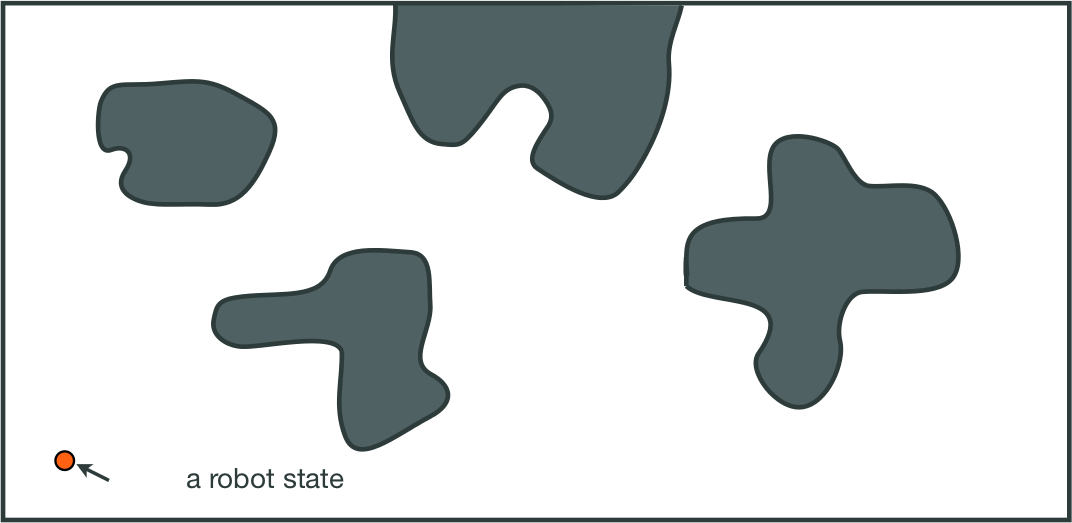
\includegraphics [width=3.75in]{state}
\caption {The 2D workspace and a single state for the point robot.}
\label {fig:prm:state}}
\end {figure}

Consider the workspace in Figure \ref{fig:prm:state}.  This image shows a
bounded workspace for the point robot in which the shaded regions are obstacles.
One particular state for the robot is highlighted.  The {\tt PRM} works by
uniformly sampling the free state space and making connections between the
samples to form a roadmap of the free state space.  The roadmap can be stored
efficiently as a graph data structure where the random samples compose the
vertices, as in Figure \ref{fig:prm:samples}.  It should be noted that the free
state space is almost never explicitly known in sampling-based methods. Each
sample that is generated is checked for collision, and only collision free
samples are retained. Additionally, there are many different ways to sample the
free state space, and changing the sampling strategy is beneficial in many
planning instances.

\begin {figure} [h]
\centering
{
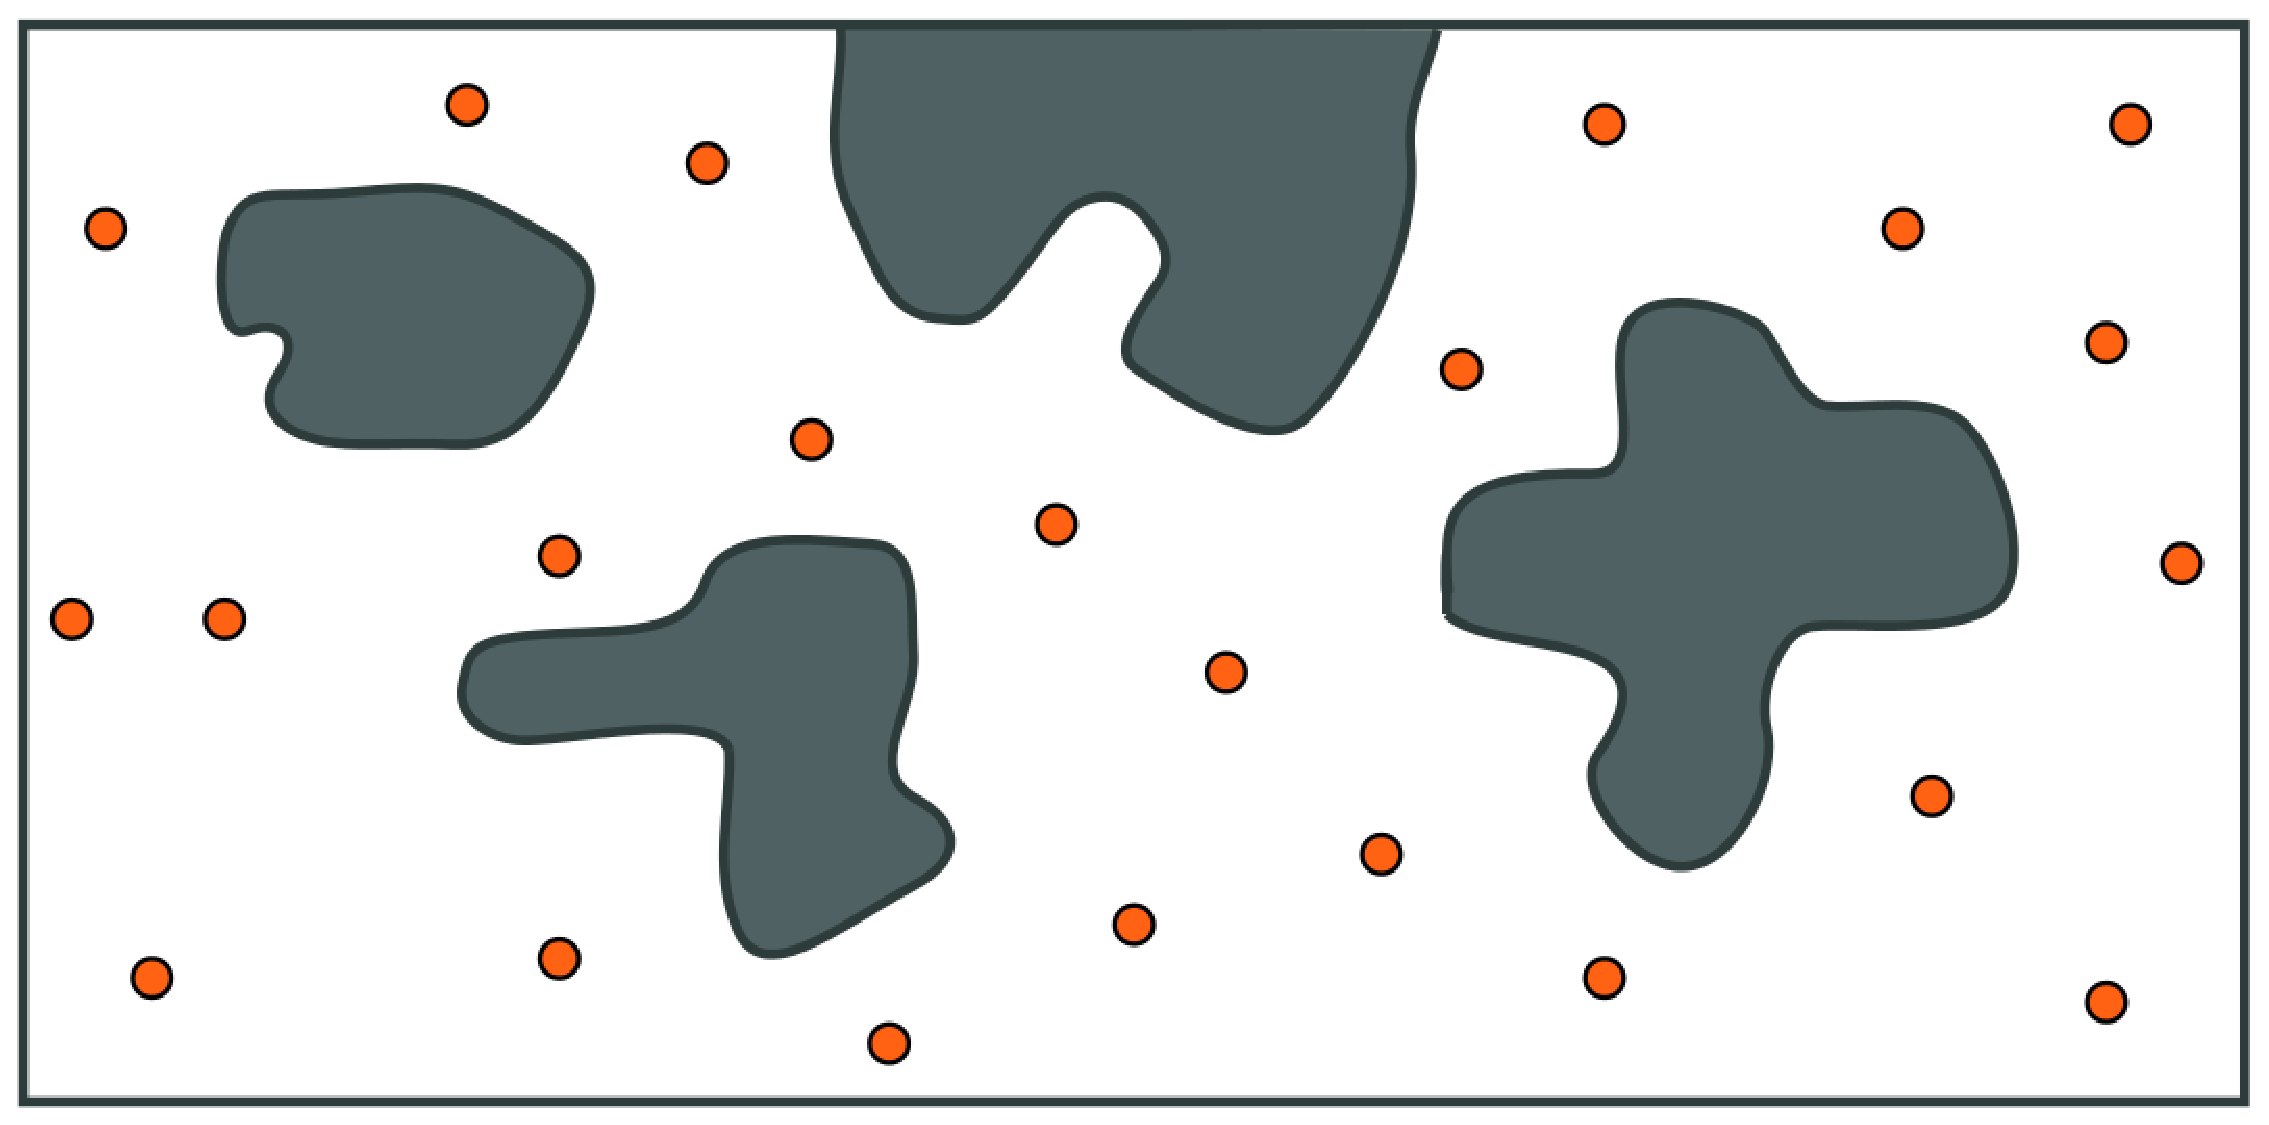
\includegraphics [width=3.75in]{samples}
\caption {One possible set of uniform random samples of the free state space}
\label {fig:prm:samples}
}
\end {figure}

Once the desired number of free samples have been found, the roadmap itself can
be constructed by connecting the random samples to form edges.  The
canonical {\tt PRM} attempts to connect each sample to the $k$ samples nearest
to it by using a local planner that is tasked with finding short collision free
paths. The local planner finds this path by interpolating the motion of the
robot between the two samples, checking for collisions at some prescribed
resolution.  If no configuration of the robot between the samples collides with
an obstacle, then an edge is inserted to the roadmap.  Figure \ref
{fig:prm:localplanner} shows a complete probabilistic roadmap in the 2D
workspace example.

\begin {figure}[h]
\centering
{
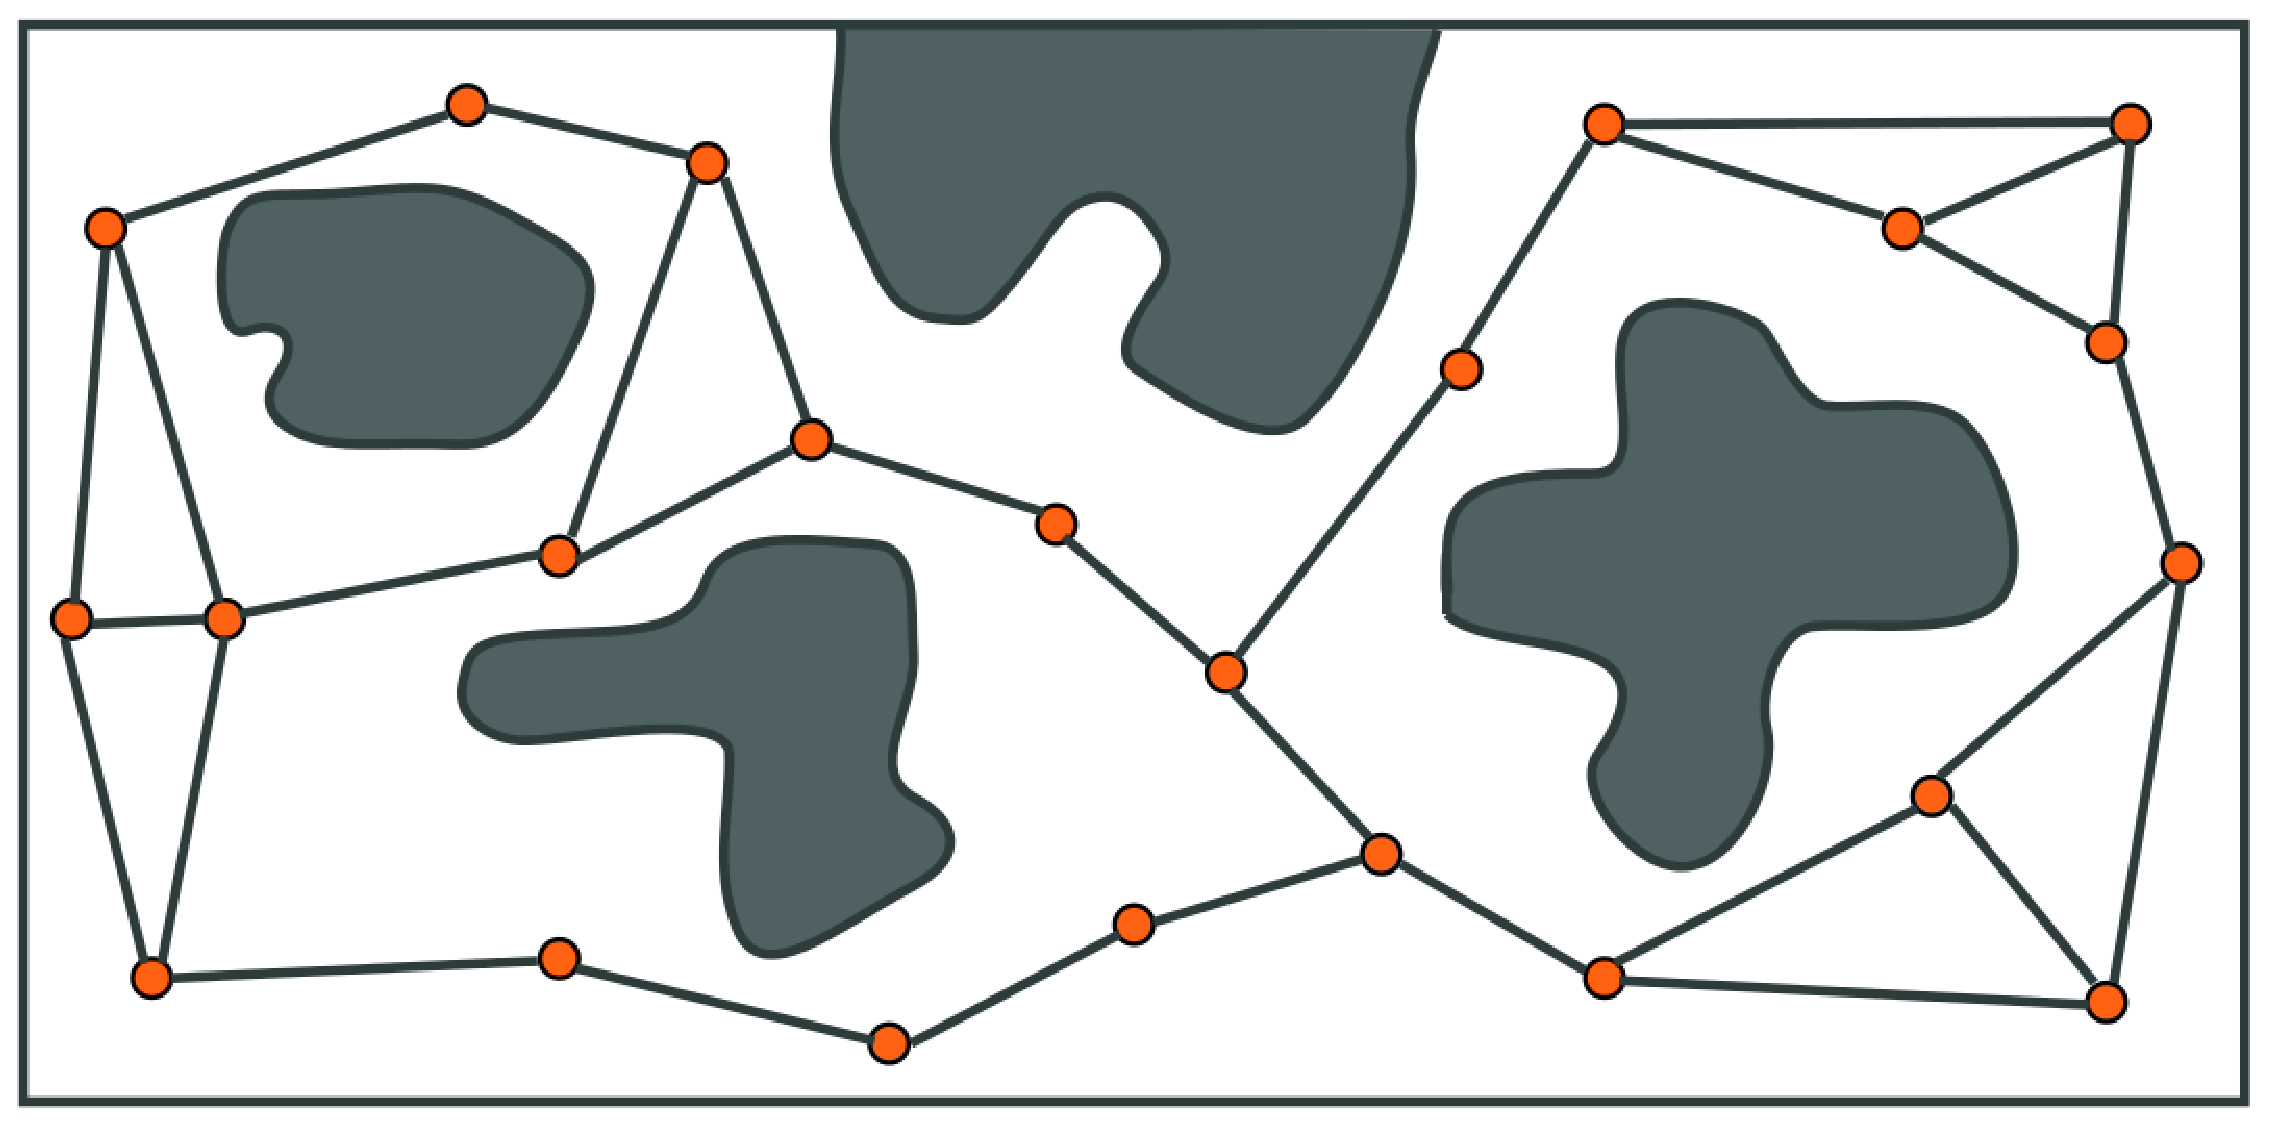
\includegraphics [width=3.75in]{localplanner}
\caption {Using a local planner, the {\tt PRM} is formed by connecting samples
that are close to one another using a straight path in the free state space.}
\label {fig:prm:localplanner}
}
\end {figure}

Once the roadmap is complete, it can be used to answer motion planning queries
by connecting the start and goal states to the roadmap using the local planner,
and performing a graph search to find the shortest path in the roadmap.  This
is seen in Figure \ref {fig:prm:query}.

\begin {figure}[h]
\centering
{
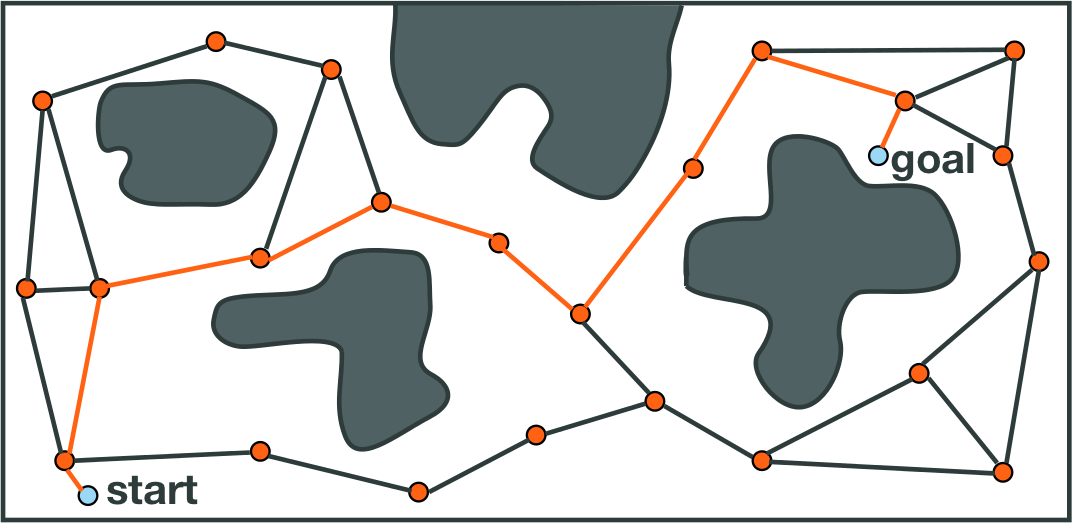
\includegraphics [width=3.75in]{query}
\caption {An example of a motion planning query on a {\tt PRM}.  The start and
the goal are connected to the roadmap, and the shortest path in the graph is
found.}
\label {fig:prm:query}
}
\end {figure}

\subsection {Tree-based Planners}
There exist many types of sampling-based planners that create tree structures
of the free state space.  The trees generated by these methods are analogous to
the probabilistic roadmap, except that the structure contains no cycles.  Due to
the wide variety of tree-based planners (e.g., {\tt RRT}\cite {LaValle:2001},
{\tt EST}\cite{Hsu:1999}, {\tt SBL}\cite{Sanchez:2003},
{\tt KPIECE}\cite{Sucan:2011}), one specific type will not be discussed in 
detail here.  However, a general framework will be described.  These methods 
begin by rooting a tree at the starting configuration of the robot.  With the 
first node of the tree intact, random sampling of the free space then occurs.  
The planner employs an expansion heuristic, which typically gives the method its 
name, from which the sample is connected to the tree along a collision free 
path.  Figure \ref{fig:tree:start} shows an example in the 2D workspace scenario
where the first few valid samples are connected to the tree.

\begin {figure}[h]
\centering
{
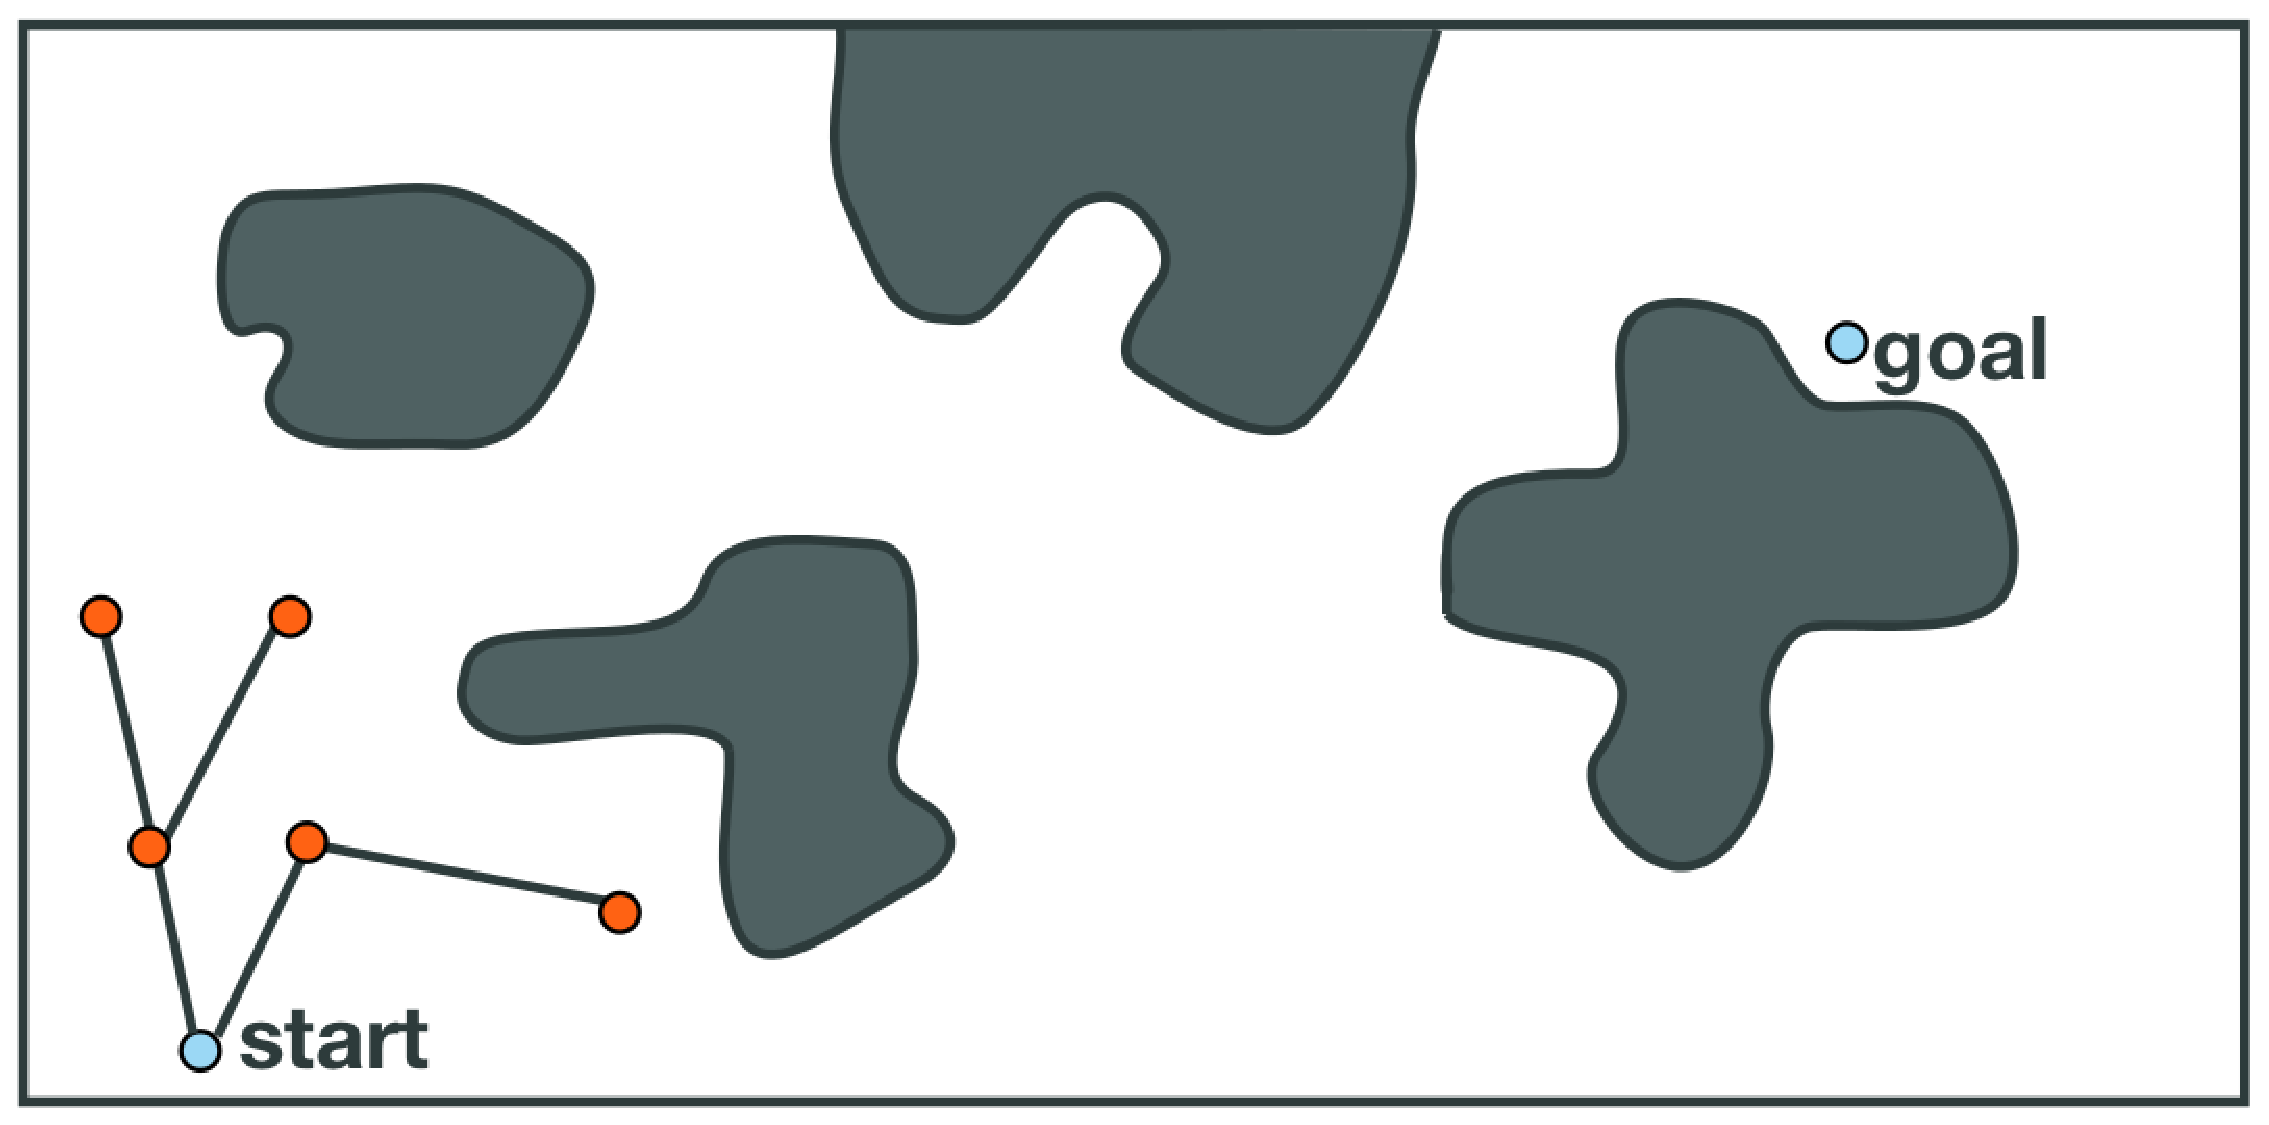
\includegraphics [width=3.75in]{tree-start}
\caption {The sampling observed after the first few samples have been connected.
Random samples are connected to the tree using an expansion heuristic.}
\label {fig:tree:start}
}
\end {figure}

Since it is highly improbable that the sampling process will ever sample the
goal state exactly, the methods often bias the expansion of the tree toward
the goal state.  If it is possible to connect the goal to the existing
tree, then the search is complete; a path through the free state space has been
found from the start to the goal.  Figure \ref{fig:tree:badgoal} shows a case
where the goal cannot be connected to the tree, and Figure \ref{fig:tree:goal}
shows the case where the goal is connected, terminating the search.

\begin {figure}[h]
\centering
{
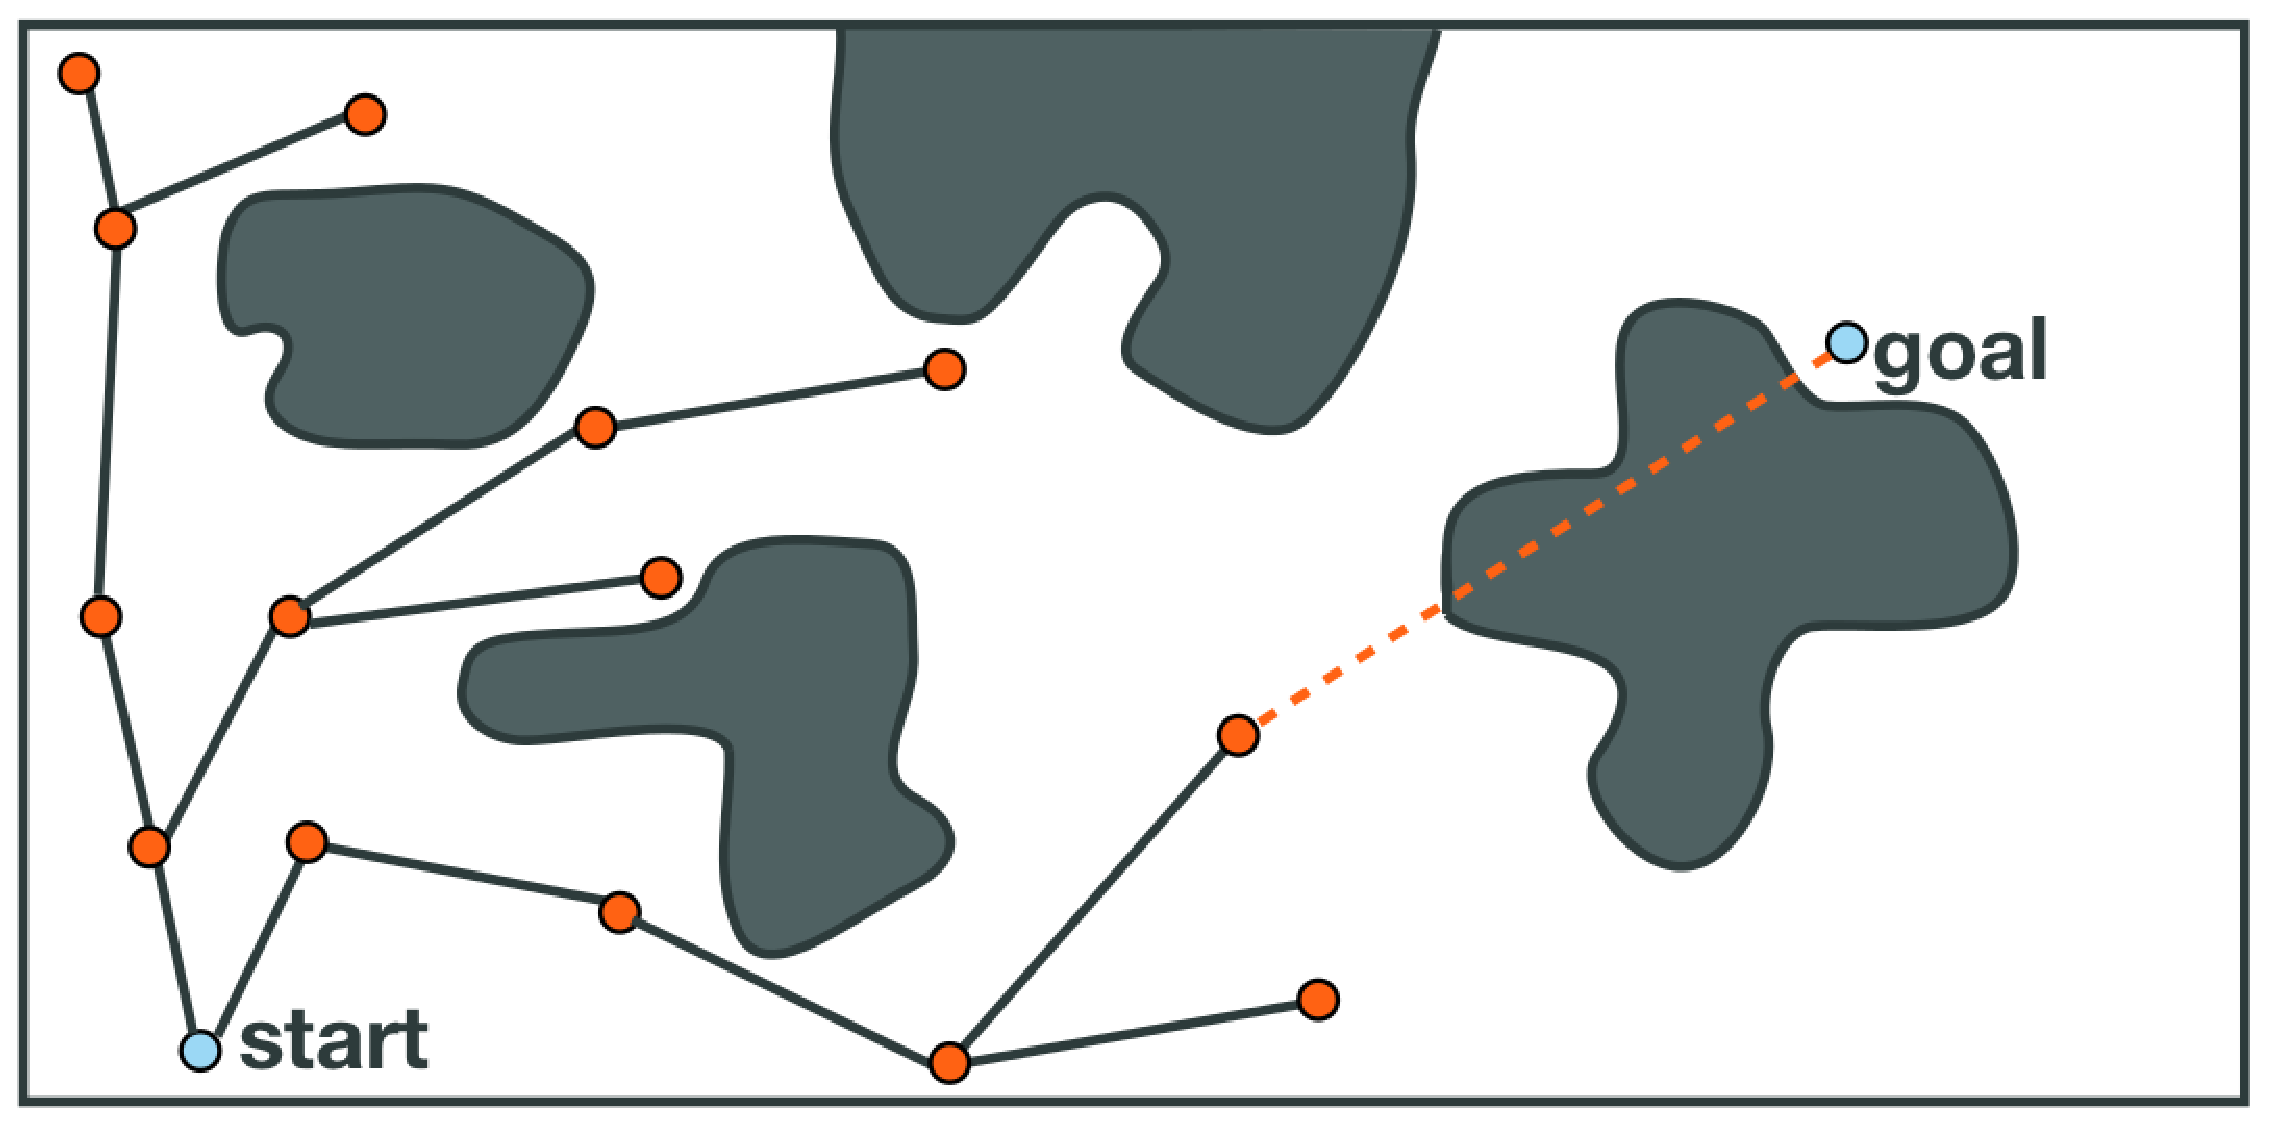
\includegraphics [width=3.75in]{tree_badgoal}
\caption {Scenario where the goal is selected during the sampling process, but
cannot be connected to the tree.  The closest node in the tree is obscured by
an obstacle.}
\label {fig:tree:badgoal}
}
\end {figure}

It is important to highlight the difference between the roadmap-based planners
and the tree-based planners. The tree-based techniques are most suitable for
single-query planning.  These trees do not normally cover the free space in the
same manner that a roadmap would.  However, when planning with differential
constraints, it is not easy to encode control information into an undirected edge.
Controls are usually directed commands, and require a specific pre-condition in
order for a particular control to be valid.  Tree-based methods, on the other
hand, excel at planning with complex dynamics because of the directed, acyclic
nature of the underlying data structure.  Control information can be encoded
for each edge of the tree, with the vertices of the tree satisfying the
prerequisites for the valid controls.

\begin {figure}[h]
\centering
{
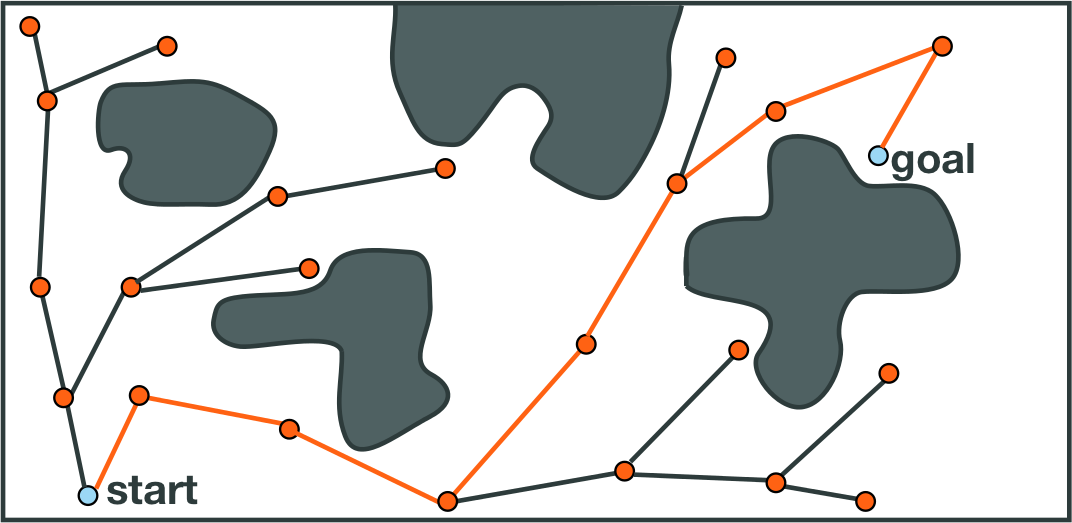
\includegraphics [width=3.75in]{tree_goal}
\caption {Scenario where the goal is selected during the sampling process, and
is connected to the tree, ending the search.}
\label {fig:tree:goal}
}
\end {figure}

Finally, it should be noted that many sampling-based approaches require a 
smaller memory footprint than other motion planners.  The compactness of these
planners stems from the sampling process itself, as well as the fact that no
explicit representation of the state space is needed in order to solve the
problem.  Storage and search of the underlying data structure (e.g., graph, tree)
should be efficient to fully maximize the quality of these methods.  However,
as tree planners are used for increasingly difficult problems, memory requirements
may increase in order to keep information that guides the expansion of the
search.

%\clearpage
\subsection {Primitives of Sampling-based Planning}
Sampling-based planning is a very powerful tool for planning in high-dimensional
spaces or for system with complex dynamics.  There exists many kinds of
sampling-based motion planners, with many commonalities, but the method in which
one samples the state space is key to computing a solution.

Collision checking is a very important part of sampling-based planning.  It is
used not only in the local planner when attempting to find collision free paths
between samples, but also during the sampling process itself.  In a complex or
high-dimensional system it may not be easy to explicitly represent the free
state space, but in sampling-based methods it is not necessary to create this
space.  It is the job of the collision checker to accept a configuration of the
robot and quickly determine whether or not this state is in collision.

Nearest neighbor searching is another cornerstone of sampling-based methods.
It is from the ability of determining whether two states of the robot are close
that many of the common approaches are able to effectively find paths through a
high-dimensional space.  Distances, however, are not easy to compute in
non-Euclidean spaces where many of the interesting problems reside.  Kd-trees
offer one way to perform this search, but the optimal connection strategy for
samples remains elusive.

The core OMPL library cleanly implements all of these primitives of
sampling-based motion planning.  Chapter \ref{chp:ompl.app} shows how the
planners bundled with OMPL can be used to directly solve motion planning
queries, and Chapter \ref{chp:ompl} details how these primitives map to concepts
within the open motion planning library.

